%% eval.tex
%% $Id: eval.tex 5 2005-10-10 20:55:48Z bless $

\chapter{Evaluation}
\label{ch:Evaluation}

Zu Beginn der Evaluation wurde eine Nutzerstudie durchgeführt, womit ein Datensatz generiert wurde. 
Anhand dieses Datensatzes wird anschließend ein Klassifikationsmodell erstellt, womit eine Vorhersage darüber getroffen wird, an welcher Stelle ein Apnoeereignis stattgefunden hat.

\section{Studienablauf}
In Abschnitt \ref{ch:Design:sec:studienplanung} wurde eine einzelne Messung einer Studie detailliert beschrieben.
Es wurden nun 7 Probanden nach dem Prinzip des \textit{Sample of Convenience} ausgewählt.

Dieser Ablauf (siehe Abb. \ref{fig_study_flow}) wurde nun pro Studienteilnehmer jeweils in den 3 Positionen durchgeführt, womit fast alle Schlaflagen abgedeckt sind.
Zu Beginn der Studie fand eine kurze Einweisung statt, bei der der Proband erfuhr, was er zu tragen hat und wie er Anweisungen erhält, um dem Ablauf folgen zu können. 
Die Kamera wurde auf dem Stativ platziert und so ausgelegt, dass sie das Ohr des Probanden filmt. 
Das PSG-System wurde am Studienteilnehmer angebracht sowie alle nötigen Sensoren, die im Abschnitt \ref{ch:sa:psg} beschrieben wurden.
Nachdem die passenden eSense-Earpodaufsätze gefunden wurden, war der Aufbau der Studie beendet.

Nun wurde die Messung des PSG-Systems gestartet sowie die Smartphone-App geöffnet. 
Nach Eingabe der Nutzerinformationen kann der erste Durchgang, welcher abhängig vom Ablauf der 3 Positionen war, begonnen werden.
Durch den Start der Messung am Smartphone beginnt die Messung. 
Da zusätzlich der Ton durch das Mikrofon am eSense-Earpod mit aufgezeichnet wird, wird nach dem Start der Messung ein $4\si{\s}$ Zeitfenster gewählt, in dem der Teilnehmer in die Hände klatschen muss, um das Mikrofonsignal später synchronisieren zu können.
Nun beginnt die Aufzeichnung. Der Leiter der Studie hat bereits den Raum verlassen und alle Anweisungen werden durch die Earpods per Audiosignal ausgesprochen. 
Sofern die Messung beendet ist, tritt der Leiter der Studie wieder in den Raum und die Messung kann exportiert werden. 
Der Export beinhaltet jegliche Smartphone-Daten. Die PSG-Daten werden als eine komplette Messung am Ende der Studie exportiert.
Zudem wird die Kamera angehalten und eine neue Aufnahme kann gestartet werden.
Anschließend beginnt die nächste Position. Der Proband kann nun die neue Position einnehmen, anschließend wird per App die neue Messung gestartet.
Zum Abschluss aller 3 Positionen wird die Messung am PSG-System gestoppt und mittels eines vom PSG-System bereitgestellten Programms lässt sich die Messung als {\glqq \textit{edf}-Datei\grqq} exportieren.
Weitere Informationen zum Export der Daten und zur Synchronisation sind in Abschnitt \ref{ch:Implementierung:way_to_pipeline} zu finden.
Pro Position dauert eine Messung circa 7 Minuten, was bei 3 Positionen eine Gesamtdauer von 21 Minuten bedeutet.
Einschließlich der Instruktionszeit, dem Export nach der Messung und den Positionswechseln der Probanden beträgt die durchschnittliche Gesamtdauer einer Aufzeichnung circa 45-60 Minuten. 

\begin{figure}[ht]
    \centering
    \begin{subfigure}{0.53\textwidth}
        \includegraphics[width=1\textwidth]{study/study_proband_2_clean.png}
    \end{subfigure}
    \begin{subfigure}{0.3\textwidth}
        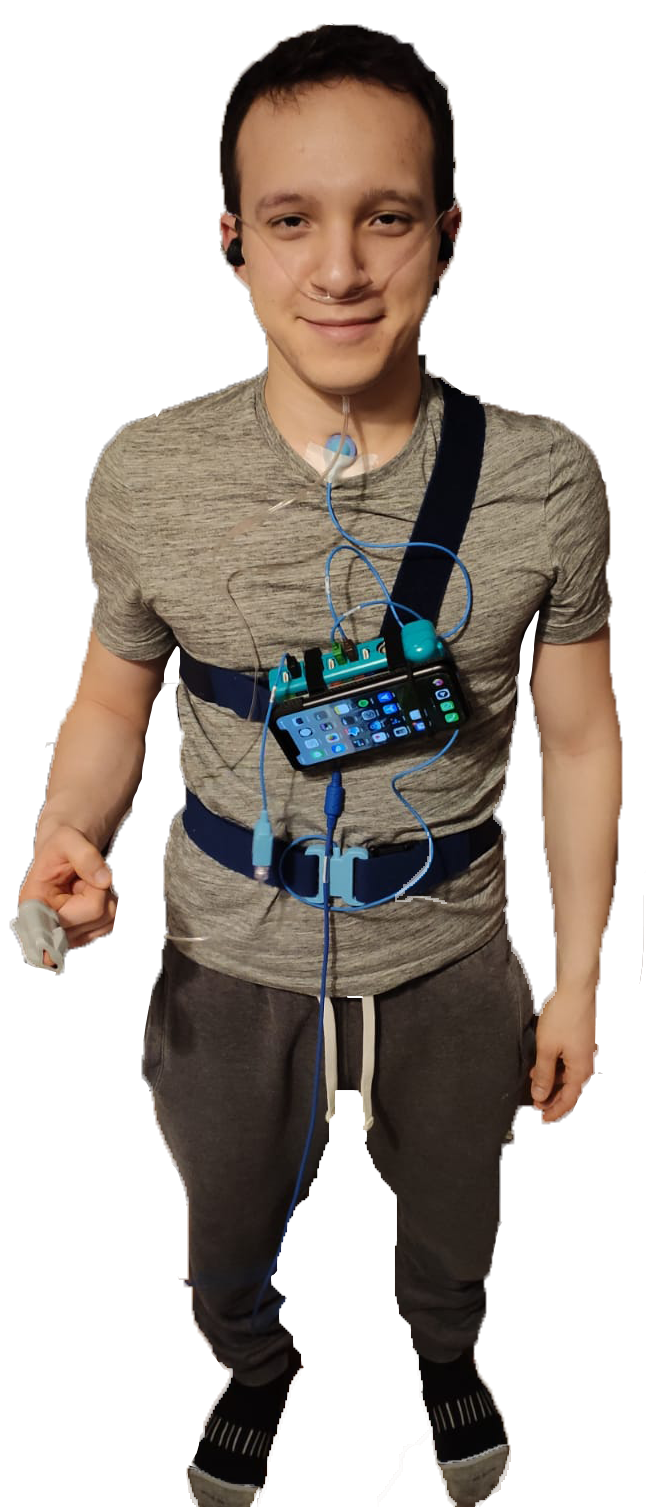
\includegraphics[width=1\textwidth]{study/study_proband_clean2.png}
    \end{subfigure}
    \caption{Darstellung von Beispielprobanden der Nutzerstudie. Das PSG-System wurde mitsamt der Sensoren am Körper angebracht. Zudem wurde das Handy am PSG-System befestigt. Die Person ist nun bereit für die erste Messung.}
    \label{implementation:study:measurement_example}
\end{figure}

Die Evaluation der Ergebnisse beginnt damit, die Daten der eSense-Earpods in Fenster (\textit{windows}) einzuteilen.
Auf diese Fenster werden anschließend \textit{Features} berechnet, welche die Grundlage für die Klassifizierung bilden.

\newpage 

\section{Gibt es passende Features?}
Die Suche nach passenden Features wird mit dem Python Package \texttt{tsfresh} angegangen, das automatisch Charakteristiken sowie deren Relevanz anhand eines Zeitintervalls berechnet \cite{TsfreshTsfresh12}.
Diese Charakteristiken werden fortan als \textit{Feature} bezeichnet.

Wie in Abschnitt \ref{ch:Implementierung:classification_pipeline} bereits erklärt, wird eine Messung in viele sich überlappende Fenster aufgeteilt. 
Eine Messung wird in Fenster der Größe von $5\si{\s}$ bzw. $10\si{\s}$ eingeteilt.
Diese Fenster sind jeweils um $1\si{\s}$ verschoben, d.h. die aneinander grenzenden Fenster überlappen sich um $4\si{\s}$ bzw. $9\si{\s}$.
Nun wird für jedes Fenster eine Featureberechnung ausgeführt, womit durch \texttt{tsfresh} ($\sim$ 6000) Features für jedes Fenster entstehen.
Als Eingabe bekommt \texttt{tsfresh} die Daten der eSense-Earpods, also die \textit{x-, y-} und \textit{z}-Achse der Gyroskop- und Beschleunigungsdaten, die mit einem Zeitstempel versehen sind. 
Die Abbildung \ref{evaluation:rawPlot} zeigt einen Ausschnitt einer Messung. 
Die in blau eingefärbte Linie stellt den absoluten Wert aus den Gyroskopdaten der $x-$, $y-$ und $z$-Achse dar.
In grün ist das Signal des direkt unter der Nase befestigten Drucksensors zu sehen, welches die Atmung repräsentiert.
Der orange markierte Bereich ist jener Bereich, in dem der Proband die Luft angehalten hat. 
Man erkennt bereits, dass die Signale während der Phase des Luftanhaltens eine geringere Amplitude im Vergleich zum Rest des Signals.
Hier sind dann deutlichere Bewegungen der Gyroskopdaten zu beobachten. 

\begin{figure}[ht]
  \centering
  \begin{subfigure}{0.7\textwidth}
      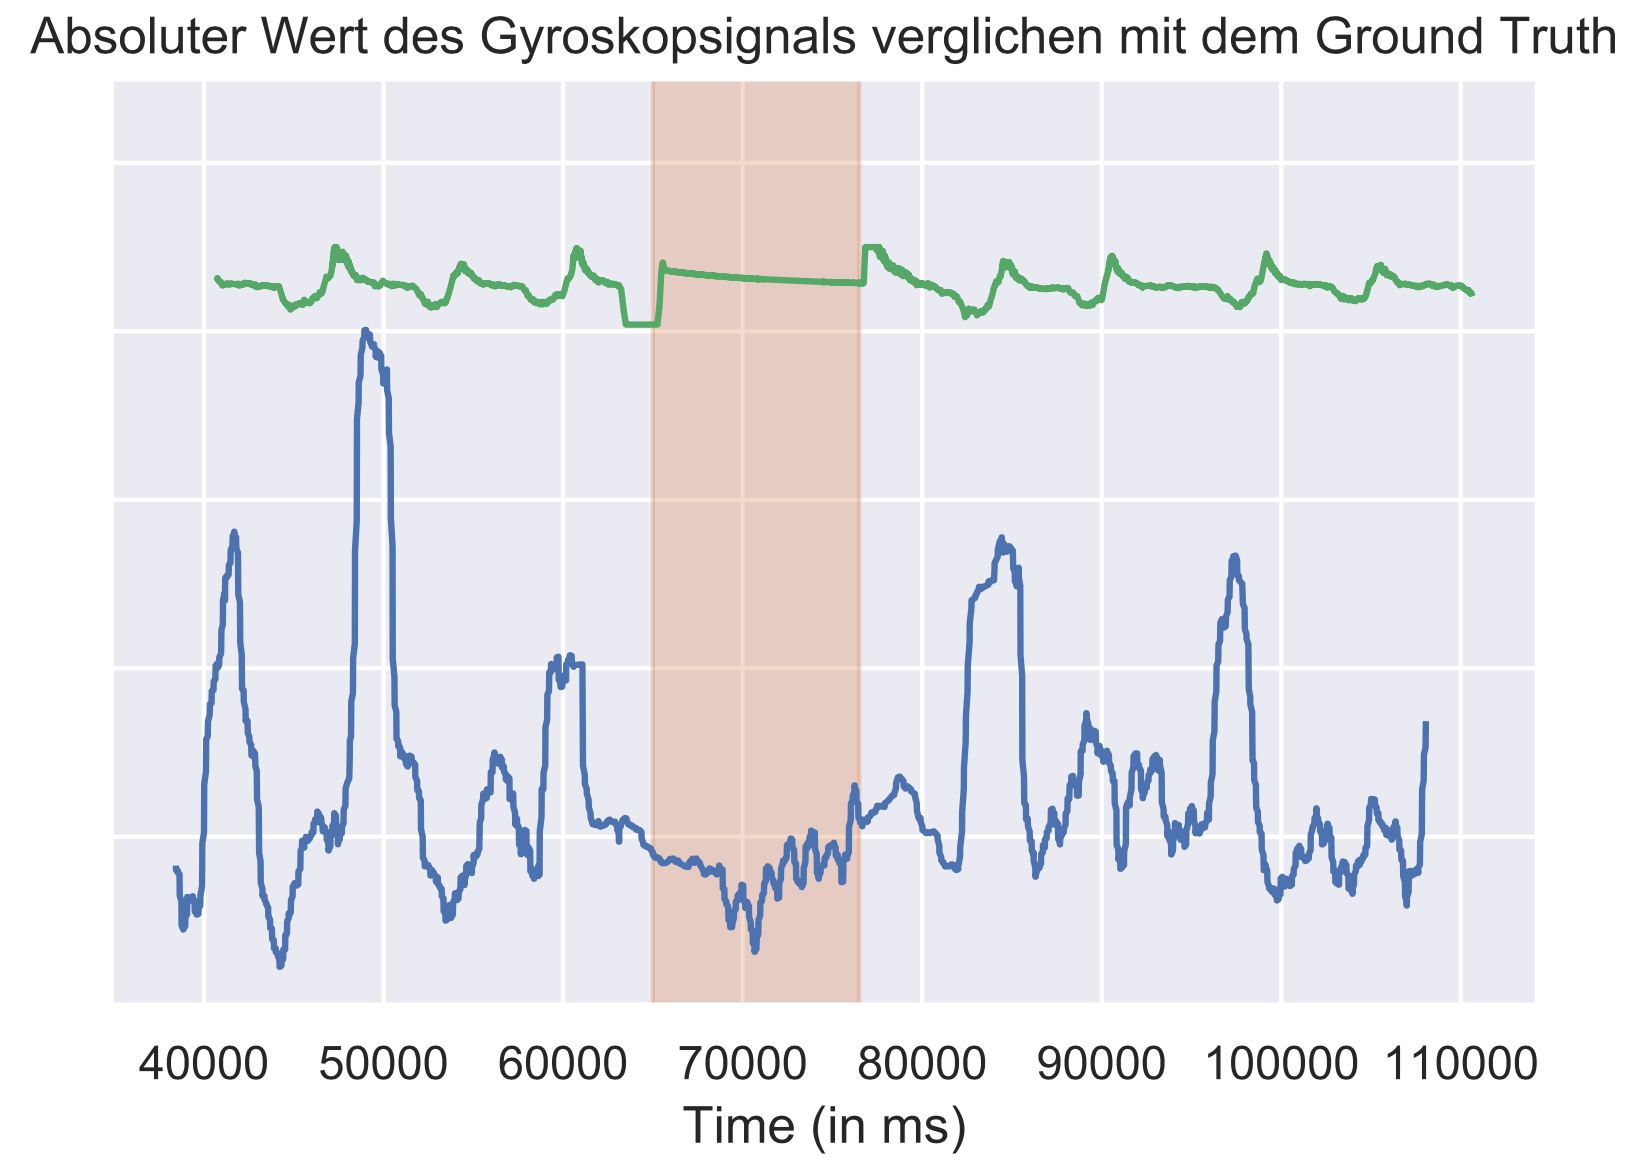
\includegraphics[width=1\textwidth]{data_analyzation/compare_raw_signal_with_flowDr_2.png}
    \end{subfigure}
  \caption{Darstellung des Signals eines Probanden während einer Messung. In grün ist das Signal des Drucksensors vom PSG-Gerät zu sehen, welcher an der Nase befestigt ist. Zudem ist der absolute Wert, welcher sich aus allen 3 Achsen des Gyroskopsignals berechnen lässt, in blau und das Apnoeereignis in orange zu sehen. Circa zwischen Sekunde 65 und 75 wurde ein Apnoeereignis simuliert. Es ist deutlich zu sehen, dass ein Apnoeereignis auch anhand der IMU-Werte zu erkennen ist. Die Berechnung des absoluten Werts ist $\sqrt{x^2+y^2+z^2}$. Beide Signale wurden normalisiert und so in der y-Achse verschoben, dass sie vergleichbar sind.}
  \label{evaluation:rawPlot}
\end{figure}

\section{Ablauf der Evaluierung}
In Abschnitt \ref{ch:Implementierung:classification_pipeline} wurde beschrieben, wie die Features berechnet und persistiert wurden. 
Nun sind pro Studienteilnehmer für alle 3 Positionen Features berechnet worden. 
Es sind jeweils die Features für ein Fenster von 5 Sekunden und 10 Sekunden berechnet worden.
Zur Erinnerung: Jede Messung wurde in Fenster der Länge von 5 bzw. 10 Sekunden aufgeteilt, wobei jedes Fenster um eine Sekunde bzw. 5 und 10 Sekunden verschoben ist.

\subsection{Data Labeling}
Bei Supervised Learning mit Klassifikation müssen die Daten bereits markiert sein, um eine Entscheidung treffen zu können. 
Beim Abspeichern der eSense Daten ist dies bereits geschehen.
Da die Messung genau vorgibt, wann eine Person die Luft anhalten soll und wann nicht, wird diese Information mit einem \textit{Boolean} als zusätzliches Attribut vermerkt.
Da bei der Klassifikation Features anhand der eSense Daten berechnet werden, darf dieses Attribut nicht Teil der Featureberechnung sein.
Bei einem 5 Sekunden Intervall werden circa 250 Einträge, bei einem 10 Sekunden Intervall circa 500 Einträge in eine Featureberechnung zusammenfließen, weshalb eine Markierung dieses Fensters gewählt werden muss.
Ist mehr als die Hälfte der Einträge positiv markiert, gilt das ganze Intervall als positiv markiert.
Dies ist eine essenzielle Entscheidung, da beim Training des Modells nun anhand dieser Markierung entschieden wird, ob ein Intervall einen Atemaussetzer repräsentiert, oder nicht.
Mit einer Grenze von 50\% wurde eine gleichwertige Aufteilung gewählt.
Nun können die Resultate mit den Klassifikatoren verglichen werden.

\subsection{Kreuzvalidierungsverfahren}
\subsubsection{Within Subject (\textit{k-fold cross validation})}
Das erste Kreuzvalidierungsverfahren ist die \textit{k-fold cross validation}.
Bei diesem Verfahren werden alle Daten in $k$ Partitionen aufgeteilt.
Eine Partition wird als Testdatensatz und die restlichen $k-1$ Partitionen werden als Trainingsdatensatz gewählt \cite{neumannMaschineLearningKIT2020}.
Somit werden alle Personen zu einem Datensatz zusammengefasst und mit der Methode \texttt{test\_train\_split} in Trainingsdaten und Testdaten aufgeteilt.
Hier wird eine Aufteilung von 70\% für die Trainingsdaten und 30\% für die Testdaten gewählt. 
Daraus ergibt sich ein \textit{score}, welcher die mittlere Genauigkeit (\textit{mean accuracy}) auf den gegebenen Testdaten, nämlich 30\% des Datensatzes, angibt.

Die Resultate sind in Tabelle \ref{evaluation:within_subject_results} zu sehen.
Die Tabelle zeigt die Ergebnisse verschiedener Klassifikationsalgorithmen mit verschiedenen Datensätzen.
Pro Klassifikationsalgorithmus wurden alle Positionen sowie jede Position einzeln betrachtet, d.h jede Position jeder Person.
Jede Kombination aus Klassifikationsalgorithmus und gewähltem Datensatz wurde nun mit den Fenstergrößen von $5\si{\s}$ und $10\si{\s}$ mit einer Verschiebung von $1\si{\s}$ und einer Verschiebung um die Fenstergröße evaluiert.
Somit wurden die Fenstergrößen mit und ohne überlappende Fenster getestet.
Die Resultate zeigen, dass der \textit{score} mit überlappenden Fenstern deutlich höher ist.
Dies könnte daran liegen, dass deutlich mehr Fenster pro Datensatz existieren, falls eine Überlappung der aneinanderfolgenden Fenster stattfindet.
Jedoch ist es auch möglich, dass Teile der überlappenden Fenster bereits erkannt und positiv markiert wurden.
Dadurch ist der überlappende Teil eventuell in den Trainingsdaten vorhanden und eine Klassifizierung ist einfach für den Klassifikationsalgorithmus.

\begin{table}[ht]
  \begin{tabular}{cc}
    \begin{minipage}{1\textwidth}
      \begin{center}
          \begin{tabular}{ | l | c | c | c | c | c | }
            \hline
            \textbf{Verfahren} & \textbf{Positionen} & \textbf{Score} & \textbf{Score} & \textbf{Score} & \textbf{Score} \\ 
            & & \textbf{$w=5\si{\s}$} & \textbf{$w=5\si{\s}$} & \textbf{$w=10\si{\s}$} & \textbf{$w=10\si{\s}$} \\
            & & \textbf{$d=1\si{\s}$} & \textbf{$d=5\si{\s}$} & \textbf{$d=1\si{\s}$} & \textbf{$d=10\si{\s}$} \\ \hline
            Random Forest & Alle &  0.87 & 0.74 & 0.89 & 0.71 \\ 
             & Rücken & 0.85 & 0.67 & 0.93 & 0.57 \\
             & Seite  & 0.86 & 0.72 & 0.89 & 0.75 \\
             & Bauch  & 0.90 & 0.85 & 0.92 & 0.66 \\ \hline
            XG Boost  & Alle & 0.88 & 0.70 & 0.92 & 0.76 \\ 
             & Rücken & 0.89 & 0.67 & 0.95 & 0.62 \\
             & Seite  & 0.90 & 0.78 & 0.92 & 0.48 \\
             & Bauch  & 0.90 & 0.75 & 0.95 & 0.63 \\ \hline
            SVM & Alle& 0.54 & 0.48 & 0.65 & 0.42 \\ 
             & Rücken & 0.60 & 0.67 & 0.72 & 0.46 \\
             & Seite  & 0.57 & 0.38 & 0.63 & 0.5 \\
             & Bauch  & 0.61 & 0.41 & 0.67 & 0.4 \\
            \hline
          \end{tabular}
      \end{center}
    \end{minipage}
  \end{tabular}

  \caption{Ergebnisse des Kreuzvalidierungsverfahrens innerhalb eines \textit{Subjects} mit einer Aufteilung von 70\% Trainings- und 30\% Testdaten. Alle Personen der Nutzerstudie wurden verwendet ($w=$ Fenstergröße, $d=$ Verschiebung der Fenster).}
  \label{evaluation:within_subject_results}
\end{table}

\subsubsection{Leave One Subject Out (LOSO)}
Neben dem $k$-fachen Kreuzvalidierungsverfahren wird das \textit{Leave One Subject Out} (\textit{LOSO}) Kreuzvalidierungsverfahren hinzugezogen. 
Hierbei wird ein Modell anhand der Daten der Studienteilnehmer trainiert, jedoch wird ein Datensatz eines Studienteilnehmers ausgelassen. 
Dieser eine Datensatz wird schließlich verwendet, um eine Vorhersage anhand der Trainingsdaten zu treffen, ohne durch interne Trainingsdaten optimiert sein zu können.
Im Folgenden wurde das LOSO Kreuzvalidierungsverfahren mit den beiden Klassifikationsalgorithmen \textit{Random Forest} und \textit{XGBoost} durchgeführt. 
Es wurde jede Person einmal ausgelassen und auf den Trainingsdatensatz vorhergesagt, welcher diese Person nicht enthält. 
Somit entstehen 7 Resultate, von denen nun der Mittelwert gebildet wurde.
Die Resultate sind in den Abbildungen \ref{evaluation:random_forest_loso:person6} und \ref{evaluation:xgboost_loso:person6} beispielhaft an Person 6 dargestellt.
Im Anhang sind weitere Abbildungen anderer Personen zu finden.
Die Abbildungen listen die Anzahl der vorhergesagten Einsen für jede einzelne Sekunde auf. 
Da eine Sekunde aufgrund der überlappenden Fenster in mehreren Fenstern vorkommt, summieren sich die Vorhersagen pro Sekunde maximal auf die Fenstergröße.
Zu Erkennen ist, dass die Fenstergröße von $10\si{\s}$ deutlich bessere Ergebnisse liefert als eine Fenstergröße von $5\si{\s}$. 
XGBoost neigt bei einer Fenstergröße von $5\si{\s}$ zum Overfitting, ebenso wie Random Forest. 
Alle Ergebnisse des LOSO Kreuzvalidierungsverfahrens sind in Form von dem jeweiligen Mittelwert von \textit{Precision} und \textit{Recall} in der darunterliegenden Tabelle mit dem daraus folgenden \textit{f1"=score} zusammengetragen.
Dieser berechnet sich mit der Formel
\[\text{\textit{f1"=score}} = 2 \cdot \frac{\text{\textit{precision}} \cdot \text{\textit{recall}}}{\text{\textit{precision}} + \text{\textit{recall}}}\text{ .}\]
Zu sehen ist, dass XGBoost bessere Ergebnisse liefert als Random Forest.
% \todo{schreibe darüber, was die ergebnisse von LOSO aussagen} \newline
Des Weiteren, um mögliche Positionsabhängigkeiten zu erkennen, wurde dasselbe erneut evaluiert, jedoch nur mit den einzelnen Positionsdaten der jeweiligen Person. 
In der Tabelle \ref{evaluation:loso_classification_results} sind die Resultate zu sehen.
%\todo{schreibe darüber, was die ergebnisse der einzelnen personen aussagen}

\subsection{Relevante Features}
Jede Klassifikation ergab ein Resultat, welches durch einzelne Features entschieden wurde. 
Das Python-Framework \texttt{scikit-learn} beinhaltet \texttt{feature\_importances\_} und zeigt die Relevanz der einzelnen Features in einem Plot.
Um einen kleinen Überblick zu bekommen, welche Features entscheidend für die Evaluation waren, sind nun einige aufgelistet:
\begin{itemize}
    \item \texttt{gyroZ partial autocorrelation}
    \item \texttt{gytoX fft coefficient}
    \item \texttt{gyroX agg autocorrelation}
    \item \texttt{accY autocorrelation}
    \item \texttt{gyroY change quantiles }
    \item \texttt{gyroZ fft coefficient}
\end{itemize}
Diese Features wurden mittels \texttt{tsfresh} berechnet und waren bei der Klassifikation des Kreuzvalidierungsverfahrens entscheidened \cite{TsfreshTsfresh12}.

Die partielle Autokorrelationfunktion (\texttt{partial autocorrelation}) beschreibt die Abhängigkeit zwischen den Werten der Zeitreihen. 
Zudem wird ein zeitlicher linearer Zusammenhang der verschiedenen Werte gemessen.
Somit haben sich die Werte in diesem Fenster zwischen den Werten weniger verändert und ähneln somit eher den positiv markierten Trainingsdaten.

Die Schnelle Fourier"=Transformation berechnet effizient die diskrete Fourier"=Transformation.
Damit können zeitdiskrete Signale in Frequenzanteile zerlegt werden. 
Es wird eine Darstellung, bestehend aus einem Zeit- und Abtastwert, in eine neue Darstellung, bestehend aus einem Frequenzanteil, einer Amplitude und einer Phase, überführt.
Die Funktion \texttt{fft\_coefficient} in \texttt{tsfresh} berechnet die Fourier Koeffizienten einer eindimensionalen diskreten Fouriertransformation für eine reale Eingabe mit dem Algorithmus der Fast-Fourier-Transformation:
\[A_k = \sum_{m=0}^{n-1} a_m \exp ^ {-2\pi i \frac{mk}{n}}, \hspace{1cm} k = 0,\dots,n-1.\]
Die bei der Apnoephase geringe Amplitude ist hier erkennbar und detektierbar, womit eine Klassifikation ermöglicht wird.

Die Aggregation \texttt{agg\_autocorrelation} berechnet den Wert der Autokorrelationsfunktion $f_{agg}$ (beispielsweise die Varianz oder den Mittelwert) über die Autokorrelation $R(l)$ für die verschiedenen Fenster. 
\[R(l) = \frac{1}{(n-l)\sigma ^2} \sum_{t=1}^{n-l} (X_t - \mu) (X_{t+l} - \mu)\]
$X_i$ sind hierbei  die Werte der Zeitreihe (\textit{Timeseries}), $n$ deren Länge, $\sigma$ und $\mu$ sind Schätzwerte für die Varianz und den Mittelwert.

Ein weiteres Feature, welches ausschlaggebend für die Klassifikation ist, ist der Wechsel der Quantilwerte (\texttt{change\_quantiles}).
Pro Fenster wird ein niedriges Quantil $q_l$ und ein hohes Quantil $q_h$ berechnet. 
Anschließend wird der durchschnittliche, absolute Wert der aufeinanderfolgenden Änderungen der Reihe $x$ innerhalb dieser Quantile berechnet.
Dadurch werden starke Veränderungen deutlich.
Dies zeigt, dass in diesem Fenster keine Apnoe stattfindet. 

\subsection{Vorverarbeitung durch einen Tiefpassfilter}
Als weiterer Versuch wurde ein Tiefpassfilter auf die Gyroskop- und Beschleunigungsdaten angewandt. 
Im Anschluss wurden Features mittels \texttt{tsfresh} auf jedem Fenster berechnet.
Da \texttt{tsfresh} ebenfalls Tiefpassfilter zur Featureberechnung nutzt, ergaben sich mit \textit{Random Forest} und \textit{XGBoost} schlechtere Resultate.
Dies ist darauf zurückzuführen, dass durch den Tiefpassfilter Informationen verloren gehen, welche in der Featureberechnung anschließend nicht mehr zur Verfügung stehen. 

%%%%%%%%%%%%%%%%%%%        RANDOM FOREST 5 sec %%%%%%%%%%%%%%%%%%%%%%%%%%%%%%%%%
\begin{figure}[ht]
  \textbf{Random Forest ($w=5\si{\s}$, $d=1\si{\s}$)}
    \centering
    \begin{subfigure}{1\textwidth}
        \includegraphics[width=1\textwidth]{evaluation/loso_5sec/random_forest_loso/Random Forest (Leave one Subject out: Person 6 back).png}
        %\caption{Resultate der Person 6 auf dem Rücken liegend.}
      \end{subfigure}
      \begin{subfigure}{1\textwidth}
        \includegraphics[width=1\textwidth]{evaluation/loso_5sec/random_forest_loso/Random Forest (Leave one Subject out: Person 6 side).png}
        %\caption{Resultate der Person 6 auf der Seite liegend.}
      \end{subfigure}
      \begin{subfigure}{1\textwidth}
        \includegraphics[width=1\textwidth]{evaluation/loso_5sec/random_forest_loso/Random Forest (Leave one Subject out: Person 6 stomach).png}
        %\caption{Resultate der Person 6 auf dem Bauch liegend.}
    \end{subfigure}
    \begin{subfigure}{1\textwidth}
        \begin{center}
            \begin{tabular}{ | l | c | c | r | }
              \hline
               & precision & recall & f1-score\\ \hline
              0 & 0.92 & 0.75 & 0.83 \\ \hline
              1 & 0.4  & 0.67 & 0.5 \\
              \hline
            \end{tabular}
        \end{center}
        %\caption{Random Forest mit dem Kreuzvalidierungsverfahren (LOSO): Die Tabelle zeigt den Mittelwert aller Vorhersagen der einzelnen Personen.}
    \end{subfigure}
    \newline
    \vspace*{1 cm}
    \newline
    \textbf{Random Forest ($w=10\si{\s}$, $d=1\si{\s}$)}
    \begin{subfigure}{1\textwidth}
      \includegraphics[width=1\textwidth]{evaluation/loso_10sec/random_forest_loso/Random Forest (Leave one Subject out: Person 6 back).png}
      %\caption{Resultate der Person 6 auf dem Rücken liegend.}
    \end{subfigure}
    \begin{subfigure}{1\textwidth}
      \includegraphics[width=1\textwidth]{evaluation/loso_10sec/random_forest_loso/Random Forest (Leave one Subject out: Person 6 side).png}
      %\caption{Resultate der Person 6 auf der Seite liegend.}
    \end{subfigure}
    \begin{subfigure}{1\textwidth}
      \includegraphics[width=1\textwidth]{evaluation/loso_10sec/random_forest_loso/Random Forest (Leave one Subject out: Person 6 stomach).png}
      %\caption{Resultate der Person 6 auf dem Bauch liegend.}
  \end{subfigure}

  \begin{subfigure}{1\textwidth}
      \begin{center}
          \begin{tabular}{ | l | c | c | r | }
            \hline
             & precision & recall & f1-score\\ \hline
            0 & 0.92 & 0.76 & 0.83\\ \hline
            1 & 0.43 & 0.69 & 0.53\\
            \hline
          \end{tabular}
      \end{center}
      %\caption{Random Forest mit dem Kreuzvalidierungsverfahren (LOSO): Die Tabelle zeigt den Mittelwert aller Vorhersagen der einzelnen Personen.}
  \end{subfigure}
    \caption{Das Kreuzvalidierungsverfahren (LOSO) mit dem Klassifikationsalgorithmus Random Forest. Das Modell wurde auf allen Personen, exklusive einer Person, trainiert. Auf alle Positionen dieser einen Person wurde eine Vorhersage getroffen. Die Grafiken stellen die Resultate von Person 6 dar. Die blauen Bereiche sind die, in denen die Luft angehalten wurde, die orange Kurve zeigt die Vorhersage ($w=$ Fenstergröße, $d=$ Verschiebung der Fenster). Die jeweils darunter liegende Tabelle zeigt den Mittelwert der Resultate (\textit{precision} \& \textit{recall}) des Kreuzvalidierungsverfahrens aller Personen sowie der daraus berechnete \textit{f1-score}.}
\label{evaluation:random_forest_loso:person6}
\end{figure}

%%%%%%%%%%%%%%%%%%%        XG BOOST 5 sec %%%%%%%%%%%%%%%%%%%%%%%%%%%%%%%%%

\begin{figure}[ht]
  \textbf{XG Boost ($w=5\si{\s}$, $d=1\si{\s}$)}
    \centering
    \begin{subfigure}{1\textwidth}
        \includegraphics[width=1\textwidth]{evaluation/loso_5sec/xg_boost_loso/XG Boost (Leave one Subject out: Person 6 back).png}
        %\caption{Resultate der Person 6 auf dem Rücken liegend.}
      \end{subfigure}
      \begin{subfigure}{1\textwidth}
        \includegraphics[width=1\textwidth]{evaluation/loso_5sec/xg_boost_loso/XG Boost (Leave one Subject out: Person 6 side).png}
        %\caption{Resultate der Person 6 auf der Seite liegend.}
      \end{subfigure}
      \begin{subfigure}{1\textwidth}
        \includegraphics[width=1\textwidth]{evaluation/loso_5sec/xg_boost_loso/XG Boost (Leave one Subject out: Person 6 stomach).png}
        %\caption{Resultate der Person 6 auf dem Bauch liegend.}
    \end{subfigure}

    \begin{subfigure}{1\textwidth}
        \begin{center}
            \begin{tabular}{ | l | c | c | r | }
              \hline
               & precision & recall & f1-score \\ \hline
              0 & 0.93 & 0.71 & 0.8 \\ \hline
              1 & 0.35 & 0.71 & 0.47 \\
              \hline
            \end{tabular}
        \end{center}
        %\caption{XGBoost mit dem Kreuzvalidierungsverfahren (LOSO): Die Tabelle zeigt den Mittelwert aller Vorhersagen der einzelnen Personen.}
    \end{subfigure}
    \newline
    \vspace*{1 cm}
    \newline
    \textbf{XG Boost ($w=10\si{\s}$, $d=1\si{\s}$)}
    \begin{subfigure}{1\textwidth}
      \includegraphics[width=1\textwidth]{evaluation/loso_10sec/xg_boost_loso/XG Boost (Leave one Subject out: Person 6 back).png}
      %\caption{Klassifikationsresultate der Person 6. Die Messung wurde auf dem Rücken liegend durchgeführt.}
    \end{subfigure}
    \begin{subfigure}{1\textwidth}
      \includegraphics[width=1\textwidth]{evaluation/loso_10sec/xg_boost_loso/XG Boost (Leave one Subject out: Person 6 side).png}
      %\caption{Klassifikationsresultate der Person 6. Die Messung wurde auf der Seite liegend durchgeführt.}
    \end{subfigure}
    \begin{subfigure}{1\textwidth}
      \includegraphics[width=1\textwidth]{evaluation/loso_10sec/xg_boost_loso/XG Boost (Leave one Subject out: Person 6 stomach).png}
      %\caption{Klassifikationsresultate der Person 6. Die Messung wurde auf dem Bauch liegend durchgeführt.}
  \end{subfigure}

  \begin{subfigure}{1\textwidth}
      \begin{center}
          \begin{tabular}{ | l | c | c | r | }
            \hline
             & precision & recall & f1-score \\ \hline
            0 & 0.92 & 0.77 & 0.84 \\ \hline
            1 & 0.44 & 0.7  & 0.54 \\
            \hline
          \end{tabular}
      \end{center}
      %\caption{XGBoost mit dem Kreuzvalidierungsverfahren (LOSO): Die Tabelle zeigt den Mittelwert aller Vorhersagen der einzelnen Personen.}
  \end{subfigure}
    \caption{Das Kreuzvalidierungsverfahren (LOSO) mit dem Klassifikationsalgorithmus XG Boost: Das Modell wurde auf allen Personen, exklusive einer Person, trainiert. Auf alle Positionen dieser einen Person wurde eine Vorhersage getroffen. Am Beispiel hier sind die Resultate von Person 6 zu sehen. Die blauen Bereiche sind die, in denen die Luft angehalten wurde, die orange Kurve zeigt die Vorhersage ($w=$ Fenstergröße, $d=$ Verschiebung der Fenster). Die jeweils darunter liegende Tabelle zeigt den Mittelwert der Resultate (\textit{precision} \& \textit{recall}) des Kreuzvalidierungsverfahrens aller Personen sowie der daraus berechnete \textit{f1-score}.}
\label{evaluation:xgboost_loso:person6}
\end{figure}

%%%%%%%%%%%%%%%%%%%        Position based results  5 sec %%%%%%%%%%%%%%%%%%%%%%%%%%%%%%%%%
\begin{table}
  \begin{tabular}{cc}
    \begin{minipage}{1\linewidth}
      \begin{center}
          \begin{tabular}{ | l | c | c | c | c | c | r | }
            \hline
            Klassifikation & Fenstergröße & Position & & precision & recall & f1-score \\ \hline
            Random Forest & 5s & Seite & 0 & 0.84 & 0.71 & 0.77 \\ 
                          &    &       & 1 & 0.39 & 0.55 & 0.46 \\ \hline
                          &    & Rücken& 0 & 0.9  & 0.84 & 0.87 \\ 
                          &    &       & 1 & 0.46 & 0.47 & 0.46 \\ \hline
                          &    & Bauch & 0 & 0.89 & 0.67 & 0.76 \\ 
                          &    &       & 1 & 0.53 & 0.73 & 0.61 \\ \hline
            \hline
            XG Boost & 5s & Seite & 0 & 0.85 & 0.69 & 0.76 \\
                     &    &       & 1 & 0.37 & 0.54 & 0.44 \\ \hline
                     &    & Rücken& 0 & 0.89 & 0.8  & 0.84 \\ 
                     &    &       & 1 & 0.4  & 0.49 & 0.44 \\ \hline
                     &    & Bauch & 0 & 0.91 & 0.6  & 0.72 \\ 
                     &    &       & 1 & 0.45 & 0.76 & 0.57 \\ \hline
            \hline
            Random Forest & 10s & Seite & 0 & 0.89 & 0.79 & 0.84 \\ 
                          &     &       & 1 & 0.41 & 0.53 & 0.46 \\ \hline
                          &     & Rücken& 0 & 0.89 & 0.82 & 0.85 \\
                          &     &       & 1 & 0.52 & 0.48 & 0.5  \\ \hline
                          &     & Bauch & 0 & 0.94 & 0.7  & 0.8  \\
                          &     &       & 1 & 0.46 & 0.73 & 0.56 \\ \hline
            \hline
            XGBoost & 10s & Seite & 0 & 0.89 & 0.68 & 0.77 \\
                    &     &       & 1 & 0.37 & 0.62 & 0.47 \\ \hline
                    &     & Rücken& 0 & 0.89 & 0.84 & 0.86 \\
                    &     &       & 1 & 0.53 & 0.5  & 0.52 \\ \hline
                    &     & Bauch & 0 & 0.94 & 0.7  & 0.8  \\
                    &     &       & 1 & 0.51 & 0.73 & 0.6  \\ \hline
          \end{tabular}
          \smallskip
      \end{center}
      %\label{evaluation:5s:random_forest_loso_side}
  \end{minipage} 
    
  \end{tabular}
  \caption{Zu sehen sind die Klassifikationsergebnisse mit dem Kreuzvalidierungsverfahren bei einer Fenstergröße von 5 bzw. 10 Sekunden, welche um eine Sekunde verschoben wurden. Jede Person wurde einmal beim Trainieren des Modells ausgelassen. Für diese Person wurde anschließend eine Vorhersage getroffen. Das zu sehende Ergebnis ist der Mittelwert der Resultate (\textit{precision} \& \textit{recall}) des Kreuzvalidierungsverfahrens aller Personen bezüglich der jeweiligen Positionen sowie der daraus berechnete \textit{f1-score}.}
  \label{evaluation:loso_classification_results}  
\end{table}